\documentclass[12pt]{amsart}
\usepackage{amsmath}
\usepackage{tikz}
\usetikzlibrary{matrix,arrows}
\usepackage{amsfonts,amssymb,amsthm, txfonts, pxfonts,amscd}
\usepackage[stretch=10]{microtype}
%\usepackage{hyperref}
\def\struckint{\mathop{%
\def\mathpalette##1##2{\mathchoice{##1\displaystyle##2}%
 {##1\textstyle##2}{##1\scriptstyle##2}{##1\scriptscriptstyle##2}}%
\mathpalette
{\vbox\bgroup\baselineskip0pt\lineskiplimit-1000pt\lineskip-1000pt
\halign\bgroup\hfill$}
{##$\hfill\cr{\intop}\cr\diagup\cr\egroup\egroup}%
}\limits}
\usepackage{natbib}
\usepackage{color}
\usepackage{booktabs,caption,fixltx2e}
\usepackage[flushleft]{threeparttable}
\usepackage{amsmath}
\usepackage{tikz}
\usetikzlibrary{matrix,arrows}
\usepackage{amsfonts,amssymb,amsthm, txfonts, pxfonts,amscd}
\usepackage{multirow}
\usepackage{floatrow}
\usepackage{subcaption}
% Table float box with bottom caption, box width adjusted to content
\newfloatcommand{capbtabbox}{table}[][\FBwidth]

\usepackage[margin=1in]{geometry}
\usepackage{setspace}
\doublespacing

\usepackage{xr}
\makeatletter
\newcommand*{\addFileDependency}[1]{% argument=file name and extension
  \typeout{(#1)}% latexmk will find this if $recorder=0 (however, in that case, it will ignore #1 if it is a .aux or .pdf file etc and it exists! if it doesn't exist, it will appear in the list of dependents regardless)
  \@addtofilelist{#1}% if you want it to appear in \listfiles, not really necessary and latexmk doesn't use this
  \IfFileExists{#1}{}{\typeout{No file #1.}}% latexmk will find this message if #1 doesn't exist (yet)
}
\makeatother

\newcommand*{\myexternaldocument}[1]{%
    \externaldocument{#1}%
    \addFileDependency{#1.tex}%
    \addFileDependency{#1.aux}%
}
%%% END HELPER CODE

% put all the external documents here!
\myexternaldocument{fda-recurrent}


\usepackage{soul,color, mathtools, fixmath}
\usepackage{multirow}
\usepackage[shortlabels]{enumitem}
\def\pr{\mathop{\text{pr}}\nolimits}
\def\var{\mathop{\text{var}}\nolimits}
\def\cov{\mathop{\text{cov}}\nolimits}
\def\k{{\bf k}}
\def\z{{\bf z}}
\def\W{{\bf W}}
\def\Bka{{\it Biometrika}}
\def\AIC{\textsc{aic}}
\def\T{{ \mathrm{\scriptscriptstyle T} }}
\def\v{{\varepsilon}}
\def\partitionsn{\mathop{\mathcal{P}_{[n]}}\nolimits}
\def\partitionsN{\mathop{\mathcal{P}_{\infty}}\nolimits}
\def\Dmn{\mathop{{D}_{m,n}}\nolimits}
\def\symmetricn{\mathop{\mathcal{S}_{n}}\nolimits}
\def\PE{\mathop{\rm Pitman\mbox{-}Ewens}\nolimits}
\def\per{\mathop{\rm per}\nolimits}
\def\U{\mathop{\mathcal{U}_{}}\nolimits}
\def\Nb{\mathop{\mathbb{N}_{}}\nolimits}
\def\Nbb{\mathop{\mathbf{N}_{}}\nolimits}
\def\nbb{\mathop{\mathbf{n}_{}}\nolimits}
\def\Xbb{\mathop{\mathbf{X}_{}}\nolimits}
\def\fin{\mathop{\text{fin}}\nolimits}
\def\pr{\mathop{\text{pr}}\nolimits}
\def\E{\mathcal{E}}
\def\G{\mathcal{G}}
\def\deg{\text{deg}_{}}
\def\equalinlaw{=_{\mathcal{D}}}
\def\Fk{\mathop{\mathcal{F}_k^{\downarrow}}\nolimits}
\def\F{\mathop{\mathcal{F}^{\downarrow}}\nolimits}
\def\size{\mathop{\text{size}}\nolimits}
\def\Ycong{\mathop{\EY}\nolimits}
\def\EIsig{\mathop{\mathcal{E}_{\mathcal{I}}^{\sigma}}\nolimits}
\def\EY{\mathop{\mathcal{E}_{Y}}\nolimits}
\def\finp{\mathop{\fin(\mathcal{P})}\nolimits}
\def\En{\mathop{\mathfrak{E}_{[n]}}\nolimits}
\def\EN{\mathop{\mathfrak{E}_{\Nb}}\nolimits}
\def\logit{\mathop{\text{logit}_{}}\nolimits}
\def\EI{\mathop{\mathcal{E}_{\mathcal{I}}}\nolimits}
\def\ES{\mathop{\mathfrak{E}_S}\nolimits}
\def\Ifk{\mathop{{I}_{}}\nolimits}
%\def\mathcal{I}{\mathop{\mathcal{I}_{}}\nolimits}
\def\Ycong{\mathop{\EY}\nolimits}
\def\EIsig{\mathop{\mathcal{E}_{\mathcal{I}}^{\sigma}}\nolimits}
\def\EY{\mathop{\mathcal{E}_{Y}}\nolimits}
\def\finp{\mathop{\fin(\mathcal{P})}\nolimits}
\def\En{\mathop{\mathfrak{E}_{[n]}}\nolimits}
\def\EN{\mathop{\mathfrak{E}_{\Nb}}\nolimits}
\def\logit{\mathop{\text{logit}_{}}\nolimits}
\def\EI{\mathop{\mathcal{E}_{\mathcal{I}}}\nolimits}
\def\ES{\mathop{\mathfrak{E}_S}\nolimits}
\DeclareRobustCommand{\citeext}[1]{\citeauthor{#1} (\citeyear{#1})}
\DeclareRobustCommand{\citeint}[1]{(\citeauthor{#1}, \citeyear{#1})}
\newtheorem{thm}{Theorem}[section]
\newtheorem{lemma}[thm]{Lemma}
\newtheorem{prop}[thm]{Proposition}
\newtheorem{cor}[thm]{Corollary}
\newtheorem{defn}[thm]{Definition}
\newtheorem{example}[thm]{Example}
\newtheorem{meas}[thm]{Measurement}
\newtheorem{conj}[thm]{Conjecture}
\newtheorem{assumption}[thm]{Assumption}
\newtheorem{rmk}[thm]{Remark}%\endlocaldefs
% change default numbering for enumerate environment to be in parentheses
\makeatletter
\def\S{\mathcal{S}}
\def\indep{\mathrel{\rlap{$\perp$}\kern1.6pt\mathord{\perp}}}
\def\R{\mathcal{R}}
\def\H{\mathcal{H}}
\def\E{\mathbb{E}}
\def\Y{{\bf Y}}
\def\Cov{\text{Cov}}
\def\one{{\bf 1}}
\def\diag{\text{diag}}
\def\given{\, | \,}
\def\Given{\, \big | \,}
\def\Nat{\mathbb{N}}
\def\Real{\mathbb{R}}
\def\bft{{\bf t}}
\def\bfx{{\bf x}}
\def\bfp{{\bf p}}
\def\bfT{{\bf T}}
\def\bfD{{\bf D}}
\def\dotminussym#1#2{%
  \setbox0=\hbox{$\m@th#1-$}%
  \kern.5\wd0%
  \hbox to 0pt{\hss\hbox{$\m@th#1-$}\hss}%
  \raise.6\ht0\hbox to 0pt{\hss$\m@th#1.$\hss}%
  \kern.5\wd0}
\newcommand{\dotminus}{\mathbin{\mathpalette\dotminussym{}}}
\DeclareMathOperator*{\argmax}{arg\,max}
\DeclareMathOperator*{\argmin}{arg\,min}
\mathchardef\mhyphen="2D
% display breaks

\begin{document}

\title[Supplement to ``Recurrent event analysis with functional covariates via random subsampling'']{Supplementary Materials to ``Recurrent event analysis in the presence of real-time high frequency data via random subsampling''}
% \author{Walter Dempsey}
% \address {Department of Biostatistics, University of Michigan, 1415 Washington Heights, Ann Arbor, MI 48109, USA}
% \email{wdem@umich.edu}

\date{\today}

\begin{abstract}
This is the supplementary materials to the manuscript titled ``Recurrent event analysis in the presence of real-time high frequency data via random subsampling.''  Section~\ref{app:prooflemma31} contains the proofs for Lemmas~\ref{lemma:logistic}, Lemma~~\ref{lemma:simpleasym}.  Section~\ref{app:optimalweights} contains that proof of Proposition~\ref{prop:optimal}.
Section~\ref{app:extrasims} contains additional simulations and case study details.
\end{abstract}

\keywords{recurrent events; probabilistic subsampling; estimating equations; high frequency time series; logistic regression}

\maketitle

\appendix

\section{Measurement-error models with event processes}
\label{section:memproblems}

One potential criticism for~\eqref{eq:hazard} is that the health process may be measured with error. A common mathematical strategy for joint models is to consider an unobservable, latent process~$\eta_i$ such that~$\bfT_i \indep x_i \given \eta_i$, i.e., the two processes are conditionally independent given the latent trajectory. For example, take~$\eta_i$ to be a zero-mean Gaussian process with
\begin{equation}\label{eq:jm}
x_i(t) = \eta_i (t) + \epsilon_i (t),\quad \text{ and } \log h_i (t
\given \eta ) = \log h_0 (t) + g_t \left( H_{i,t}^N \right)^{\prime}
\alpha + \int_{t-\Delta}^t \eta_i (s) \beta (s) ds
\end{equation}
where~$\epsilon_i(t)$ is a white-noise measurement error term. Thus, $\eta_i (t)$ is the ``true and unobserved value of the longitudinal outcome'' \citep[Sec. 2.1, pp.3]{Rizopoulos2010}. The conditional survival function of the $j$th event~$T_j$ given~$\bfx_i$ and all prior events~$\bfT_{-j} := \{ T_1, \ldots, T_{j-1} \}$ is
\[
\pr \left ( T_j > t+s \Given \H_{i,\tau_i}^X, \bfT_{-j} = \bft_{-j}, T_j > t \right) = E \left( - \exp \left( \int_{t}^{t+s} h_i (u \given \eta ) du \right) \Given \bfx_i, \bfT_{-j} = \bft_{-j} \right),
\]
where the expectation is a Gaussian integral, albeit infinite-dimensional.  For most choices of covariance structure, if the white-noise error term is non-zero then the above calculation will show the conditional survival function depends not only on past $x$-values, but also on future $x$-values, i.e.,~$\bfx$ and~$\bfT$ do not satisfy \emph{independent evolution}~\citep{DempseyPMCC2}. This is quite unnatural, as~\eqref{eq:jm} suggests the instantaneous risk of an event at time~$t$ depends on future values of the sensor process. To ensure independent evolution, we set~$\epsilon (t) \equiv 0$ and treat~$\bfx_i$ as a Gaussian process measured without a white-noise error term.
Our procedure will only rely on the Gaussian assumption when~$\bfx$ is not fully observed; see Section~\ref{section:missingdata} for details on handling of missing data.


\section{Derivation of the design-unbiased score equations}
\label{app:prooflemma31}

\begin{proof}[Proof of Lemma~\ref{lemma:logistic}]
Recall~$\frac{d}{d\theta} \log h_i (t; \theta) = \frac{h^{(1)}_i (t; \theta)}{h_i (t; \theta)}$. Under the log-linear intensity function given by~\eqref{eq:approx_hazard}, $\frac{d}{d\theta} \log h_i (t; \theta) = W_{i,t}$ and
\[
\frac{d}{d \theta} \log \left( \pi_i (t) + h_i (t;\theta) \right) =
\frac{\exp \left( W_{i,t}^\top \theta \right)}{\pi_i (t) + \exp
  \left( W_{i,t}^\top \theta \right)} W_{i,t}
\]
Therefore,
\begin{align*}
\tilde U_n (\theta)
  &= \sum_{i=1}^n \left \{ \sum_{t \in \bfT_i} W_{i,t} - \sum_{t \in \bfT_i \cup \bfD_i} \frac{\exp \left( W_{i,t}^\top \theta \right)}{\pi_i (t) + \exp \left( W_{i,t}^\top \theta \right)}  W_{i,t} \right \} \\
  &= \sum_{i=1}^n \left \{ \sum_{t \in \bfT_i} \frac{\pi_i (t)}{\pi_i (t) + \exp \left( W_{i,t}^\top \theta \right)} W_{i,t} - \sum_{t \in \bfD_i} \frac{\exp \left( W_{i,t}^\top \theta \right)}{\pi_i (t) + \exp \left( W_{i,t}^\top \theta \right)} W_{i,t} \right \} \\
  &= \sum_{i=1}^n \left \{ \sum_{t \in \bfT_i} w_{i} (t; \theta) W_{i,t} -
    \sum_{t \in D_i} (1 - w_i (t; \theta)) W_{i,t} \right \} \\
  &= - \sum_{i=1}^n \sum_{t \in \bfT_i \cup \bfD_i} \left[ {\bf 1} [t \in \bfD_i]  - w_{i} (t; \theta) \right] W_{i,t} \\
  &= \sum_{i=1}^n \sum_{t \in \bfT_i \cup \bfD_i}
    \left[ {\bf 1} [t \in \bfD_i]  - \frac{1}{1 + \exp\left( - (
          \tilde W_{i,t}^\top \theta + \log (\pi_i (t) ) ) \right)}
    \right] \tilde W_{i,t}.
\end{align*}
where~$\tilde W_{i,t} = - W_{i,t}$. This is exactly the score equation
for logistic regression with offset~$\log \pi_i (t)$.
\end{proof}

\begin{proof}[Proof of Lemma~\ref{lemma:simpleasym}]
% Lemma~\ref{lemma:simpleasym} will be proven under regularity conditions A-E in~\cite[pp. 420--421]{Andersen1993} along with the following assumptions related to the subsampling rate~$\pi_i (t)$.
Define the joint counting process
\[
M_i (t) = N_i (t) - \int_0^t (h_i (s; \theta) + \pi_i (s)) R_i (s) ds.
\]
where~$N_i (t)$ is the counting process with jumps at all~$t \in \bfT_i \cup \bfD_i$. Asymptotic consistency is guaranteed~\cite[Theorem VI.1.1]{Andersen1993} if
\begin{equation}
\label{eq:andersen1}
n^{-1} \tilde U_n (\theta_0 ) \overset{P}{\to} 0,
\end{equation}
and
\begin{equation}
\label{eq:andersen2}
n^{-1} \frac{d}{d \theta^{\top}} \tilde U_n (\theta) \big |_{\theta =
  \theta_0} = \Xi (\theta),
\end{equation}
and
\begin{equation}
\label{eq:andersen3}
\lim_{n \to \infty} P \left( \left | n^{-1} \frac{d^2}{d \theta_j d
      \theta_k} \tilde U_n (\theta) \right | < M \text{ for all }
  j,k \text{ and all } \theta \in \Theta_0 \right) = 1
\end{equation}
To prove~\eqref{eq:andersen1}, we decompose~$\tilde U_n (\theta_0)$ into
three terms
\begin{equation}
\label{eq:decomp}
n^{-1} \tilde U_n (\theta_0) = n^{-1} U_n (\theta_0 )  + n^{-1} \left(
  \hat U_n (\theta_0) - U_n (\theta) \right) + n^{-1} \left(\tilde U_n
  (\theta_0) - \hat U_n (\theta_0) \right)
\end{equation}
where, recall,~$\hat U_n (\theta_0)$ are the logistic score equations with $\int_0^\infty X_i(t,s) \beta(s) ds$ and~$\tilde U_n (\theta_0)$ with the approximation~$C_{i,t}^\top J_{\phi, \psi} {\bf b}$. \cite{Andersen1993} (Theorem VI.1.1) show that~$n^{-1} U_n (\theta_0)
\to 0$. The second term
\begin{align*}
n^{-1} \left( \hat U_n (\theta_0) - U_n (\theta_0) \right) =
  \frac{1}{n} \sum_{i=1}^n \int_0^{\tau} \frac{h^{(1)} (s;
  \theta_0)}{\pi_i (s) + h (s;\theta_0)} d M_i (s).
\end{align*}
where~$h(\cdot; \theta_0)$ is given by~\eqref{eq:hazardlinear}. Lenglart's inequality implies the second term converges in probability to zero under Assumptions~\ref{E1} and~\ref{E2}. The third term satisfies
\begin{align*}
  &n^{-1} \left \| \hat U_n (\theta_0) - \tilde U_n (\theta_0) \right \| \\
  \leq & M n^{-1} \sum_{i=1}^n \sum_{t \in \bfT_i \cup \bfD_i} \bigg \| g
         \left( \tilde W_{i,t}^\top \theta  + \sum_{k=K_x+1}^\infty \hat
         c_{i,k} (t) \int_{t-\Delta}^t \hat \psi_k (s) \phi (s)^\top b
         + \log (\pi_i (t) ) \right) - g \left( \tilde W_{i,t}^\top
         \theta + \log (\pi_i (t)) \right) \bigg \| \\
&\leq M n^{-1} \sum_{i=1}^n \sum_{t \in \bfT_i \cup \bfD_i}
    \sup_{x \in \mathbb{R}} \left \| g^\prime \left( x \right)
  \right\| \times \left \| \sum_{k=K_x+1}^\infty \hat c_{i,k} (t)
  \sum_{l=1}^{K_b} \int_{t-\Delta}^t \hat \psi_k (s) \phi_l (s) b_l
  \right \| \\
&= \frac{M}{4} n^{-1} \sum_{i=1}^n \sum_{t \in \bfT_i \cup \bfD_i}
  \sum_{l=1}^{K_b} \left \| \int_{t-\Delta}^t
  \left( X(t,s) - \sum_{k=1}^{K_x} \hat c_{i,k} (t) \psi_k (s) \right)
  \phi_l (s) b_l\right \| \\
&\to \frac{M}{4} \int_0^\tau \sum_{l=1}^{K_b} \left \| \int_{t-\Delta}^t
  \left( X(t,s) - \sum_{k=1}^{K_x} \hat c_{i,k} (t) \psi_k (s) \right)
  \phi_l (s) b_l\right \| (f_0(t) + f_1(t)) dt
\end{align*}
where~$M = \sup \| \tilde W_{i,t} \|$,~$g(x) = 1/(1+\exp(-x))$ is the
expit function.
The second inequality is due to the Taylor remainder theorem. The third is due to~$g^\prime (x) = e^x/(1+e^x)^2 \leq e^0/(1+e^0)^2 = 1/4$, reordering the summation, and rewriting the error term in terms of the difference between~$X(t,s)$ and the approximation with truncation level~$K_x$. Letting~$n \to \infty$ allows us to re-write the outside sums in terms of the integrated difference where the integral is with respect to the joint event and sampling distributions~$(f_0(t) + f_1 (t))$. Finally, under Assumptions~\ref{assumption:truncation}, \cite{Park2018} show
\[
X(t,s) - \sum_{k=1}^{K_x} \hat c_{i,k} (t) \psi_k (s) \overset{P}{\to} 0
\]
as~$K_x \to \infty$, which implies the third term goes to zero as the truncation level goes to infinity. The same argument can be used in conjunction under assumptions~\ref{E1} and~\ref{E4} to prove~\eqref{eq:andersen2}.

To prove~\eqref{eq:andersen3}, we start with equation~\eqref{eq:approxscore}, which we rewrite here for completeness:
\[
\hat{U}_n (\theta) = \sum_{i=1}^n \left[ \sum_{u \in \bfT_i} w_i(u; \theta)
  \frac{h^{(1)} (u; \theta)}{ h ( u; \theta)}  - \sum_{u \in \bfD_i} w_i(u;
  \theta) \frac{h_i^{(1)} (u; \theta)}{ \pi_i (u) } \right].
\]
Let~$N_i^{(e)} (t)$ and $N_i^{(s)} (t)$ be the event and subsampling counting processes with jumps at $t \in \bfT_i$ and $\bfD_i$ respectively.  Then
\begin{equation}
\label{eqapp:upperbound}
\left | n^{-1} \frac{d^2}{d \theta_j d \theta_k} \tilde U_n (\theta)  \right | \leq \frac{1}{n} \sum_{i=1}^n \int_0^\tau w_i (t;\theta) \times H_{in} (t) R_i (t) dN_i^{(e)} (t) +
\frac{1}{n} \sum_{i=1}^n \int_0^\tau \frac{w_i (t;\theta)}{\pi_i (t)} \times G_{in} (t) R_i (t) dN_i^{(e)} (t)
\end{equation}
where $H_{in}(t)$ and $G_{in}(t)$ are from Condition VI.1.1(E) in~\cite[pp. 421]{Andersen1993}. The first term converges in probability to a finite quantity by~\cite{Andersen1993}.  Since~$w_i(t;\theta)/\pi_i (t) = (\pi_i(t)+h_i(t;\theta))^{-1}$, the second term which simplifies to
\[
\frac{1}{n} \sum_{i=1}^n \int_0^\tau \frac{G_{in} (t)}{\pi_i (t)+h_i(t;\theta)} R_i(t) dN_i^{(e)} (t)
\leq
\frac{1}{L \cdot n} \sum_{i=1}^n \int_0^\tau G_{in} (t) R_i (t) dN_i^{(e)} (t)
\]
by Assumption~\ref{E1} (i.e., the subsampling rate is lower bounded by $L$). The right hand side is the optional variation of the local square integrable martingale
$$
\frac{1}{L \cdot n} \sum_{i=1}^n \int_0^t G^{1/2}_{in} (s) dN_i^{(e)} (s)
$$
This martingale has predicable variation process
$$
\frac{1}{L \cdot n} \sum_{i=1}^n \int_0^t G_{in} (s) \pi_i (s) R_i (s) ds
$$
Since both processes have the same limits, conditions VI.1.1(E) in~\cite{Andersen1993} and Assumption~\ref{E1} imply that the second term on the right hand side of~\eqref{eqapp:upperbound} also converges to a finite quantity as $n \to \infty$ for every $K_x$ which completes the proof.

This proves~$\hat \theta_n \overset{P}{\to} \theta_0$ as $n \to \infty$ and $K_x \to \infty$. Note that the argument holds for any choice of weight functions~$w_i (t;\theta)$; implying convergence holds more broadly for all approximate score equations in~\eqref{eq:approxscore}.
\end{proof}

\begin{proof}[Proof of Asymptotic Normality]
Consider a Taylor-expansion of $\tilde U_n (\theta)$ centered at $\theta_0$ when $\hat \theta_n \in \Theta_0$.  We can write as
\begin{align*}
\tilde U_n (\hat \theta_n) &= \tilde U_n (\theta_0) -  (\hat \theta_n - \theta_0) \frac{\partial}{\partial \theta} \tilde U_n (\theta) \mid_{\theta=\theta_0} - (\hat \theta_n - \theta_0) \sum_{l=1}^p (\hat \theta_{ln} - \theta_{l0}) \frac{\partial^2}{\partial \theta \partial \theta_l} \tilde U_n (\theta) \mid_{\theta=\theta^\star} \\
0 &= \tilde U_n (\theta_0) + (\hat \theta_n - \theta_0) \left[ \frac{\partial}{\partial \theta} \tilde U_n (\theta) \mid_{\theta=\theta_0} + \frac{1}{2} \sum_{l=1}^p (\hat \theta_{ln} - \theta_{l0}) \frac{\partial^2}{\partial \theta \partial \theta_l} \tilde U_n (\theta) \mid_{\theta=\theta^\star} \right] \\
n^{1/2} (\hat \theta_n - \theta_0) &= \left[ \frac{1}{n} \frac{\partial}{\partial \theta} \tilde U_n (\theta) \mid_{\theta=\theta_0} + \frac{1}{2n} \sum_{l=1}^p (\hat \theta_{ln} - \theta_{l0}) \frac{\partial^2}{\partial \theta \partial \theta_l} \tilde U_n (\theta) \mid_{\theta=\theta^\star} \right]^{-1} n^{-1/2} \tilde U_n (\theta_0)
\end{align*}
where~$\theta^\star$ is on the line segment between $\hat \theta_n$ and $\theta_0$. First, the term
$$
\frac{1}{n} \frac{\partial}{\partial \theta} \tilde U_n (\theta) \mid_{\theta=\theta_0} + \frac{1}{2n} \sum_{l=1}^p (\hat \theta_{ln} - \theta_{l0}) \frac{\partial^2}{\partial \theta \partial \theta_l} \tilde U_n (\theta) \mid_{\theta=\theta^\star}
\overset{P}{\to} \Xi(\theta_0)
$$
under conditions VI.1.1(A)--(E) in~\cite{Andersen1993} and Assumptions~\ref{E1}--\ref{E4}.  To see this, note the first term converges to $\Xi(\theta_0)$ while the second term is bounded in probability by $p M \| \theta^\star - \theta_0 \|$ for some finite constant~$M$ independent of~$\theta^\star$ where $\| \cdot \|$ is the Euclidean norm.  The second term therefore goes to zero since $\| \theta^\star - \theta_0 \| \to 0$ as $n \to \infty$.

We now consider $n^{-1/2} \tilde U_n (\theta_0 )$. Recall $\tilde U_n (\theta_0)$ can be decomposed into three terms as in~\eqref{eq:decomp}. Here, we assume $K_x \to \infty$ so the final term is negligible.  This leaves two terms
$$
U_n (\theta_0) = \sum_{i=1}^n \int_0^\tau \frac{h^{(1)}(u; \theta)}{h (u;\theta)} dM_i^{(e)} (t)
$$
where~$N_i^{(e)} (t)$ and $N_i^{(s)} (t)$ are the orthogonal event and subsampling counting processes with jumps at times $t \in \bfT_i$ and $t \in \bfD_i$ respectively.
and
\begin{align*}
(\hat U_n (\theta_0) - U_n (\theta_0) )
&= \sum_{i=1}^n \int_0^\tau \frac{h^{(1)}(s; \theta_0)}{\pi_i (s) + h(s; \theta_0)} dM_i (s) \\
&= \sum_{i=1}^n \int_0^\tau \frac{h^{(1)}(s; \theta_0)}{\pi_i (s) + h(s; \theta_0)} dM^{(e)}_i (s) +
\sum_{i=1}^n \int_0^\tau \frac{h^{(1)}(s; \theta_0)}{\pi_i (s) + h(s; \theta_0)} dM_i^{(s)} (s) \\
&= \sum_{i=1}^n \int_0^\tau (1-w(s;\theta_0)) \cdot \frac{h^{(1)}(s; \theta_0)}{h_i (s;\theta_0)} dM_i^{(e)} (s) +
\sum_{i=1}^n \int_0^\tau w(s;\theta_0) \cdot \frac{h^{(1)}(s; \theta_0)}{\pi_i (s)} dM_i^{(s)} (s)
\end{align*}
Taking difference with $U_n(\theta_0)$, the first term becomes
\[
\sum_{i=1}^n \int_0^\tau w(s;\theta_0) \cdot \frac{h^{(1)}(s; \theta_0)}{h_i (s;\theta_0)} dM_i^{(e)} (s)
\]

These are two orthogonal square integrable martingales with quadratic variation given by
\[
\sum_{i=1}^n \int_0^\tau w^2(s;\theta_0) \left[ \frac{h^{(1)}(s; \theta_0)}{h_i (s;\theta_0)} \right] \times \left[ \frac{h^{(1)} (s;\theta_0)}{h_i (s;\theta_0)} \right]^\top h_i (s) ds
\]
and
\[
\sum_{i=1}^n \int_0^\tau w^2(s;\theta_0) \left[ \frac{h^{(1)}(s; \theta_0)}{\pi_i (s)} \right] \times \left[ \frac{h^{(1)} (s;\theta_0)}{\pi_i (s)} \right]^\top \pi_i (s) ds
\]
respectively.  Using the definition $w(s;\theta_0) = \pi_i(s) / (\pi_i(s)+h_i(s;\theta_0))$, we have
\begin{align*}
&\frac{1}{n} \sum_{i=1}^n \int_0^\tau w^2(s;\theta_0) \left[ \frac{h^{(1)}(s; \theta_0)}{h_i (s;\theta_0)} \right] \times \left[ \frac{h^{(1)} (s;\theta_0)}{h_i (s;\theta_0)} \right]^\top h_i (s) ds \\
&+
\frac{1}{n} \sum_{i=1}^n \int_0^\tau w^2(s;\theta_0) \left[ \frac{h^{(1)}(s; \theta_0)}{\pi_i (s)} \right] \times \left[ \frac{h^{(1)} (s;\theta_0)}{\pi_i (s)} \right]^\top \pi_i (s) ds \\
=& \frac{1}{n} \sum_{i=1}^n \int_0^\tau w^2(s;\theta_0) \frac{h^{(1)}(s; \theta_0) [h^{(1)} (s;\theta_0)]^\top}{h_i (s;\theta_0)} \left[ 1 + \frac{h(s;\theta_0)}{\pi_i (s)} \right] ds \\
=& \frac{1}{n} \sum_{i=1}^n \int_0^\tau w^2(s;\theta_0) \frac{h^{(1)}(s; \theta_0) [h^{(1)} (s;\theta_0)]^\top}{h_i (s;\theta_0)} \left[ \frac{\pi_i (s) + h(s;\theta_0)}{\pi_i (s)} \right] ds \\
=& \frac{1}{n} \sum_{i=1}^n \int_0^\tau w(s;\theta_0) \frac{h^{(1)}(s; \theta_0) [h^{(1)} (s;\theta_0)]^\top}{h_i (s;\theta_0)} ds
\to \Xi (\theta_0).
\end{align*}
Returning to the Taylor-expansion, under conditions VI.1.1(A)--(E) in~\cite{Andersen1993} and Assumptions~\ref{E1}--\ref{E4}, we can apply Rebolledo's martingale central limit theorem so that
$$
\sqrt{n} (\hat \theta_n - \theta_0) \overset{D}{\to} N(0, \Xi(\theta_0) ^{-1} \times \Xi(\theta_0) \times \Xi(\theta_0) ^{-1} )
$$
which completes the proof.
\end{proof}

% \section{Penalized logistic mixed-effects model}
% \label{app:penlogit}

% Here we derive a penalized adaptive Gaussian quadrature (PADQ) to fit the   penalized logistic mixed-effects model.  Here, for clarity, we write $Y_{ij} \in \{ 0, 1 \}$ to be the sequence of binary indicators for participant $i = 1,\ldots,n$ and $j$ indexes the event and subsampled times.  We write $W_{ij}$ to denote the time-varying covariate.  Then the score equations for the penalized logistic regression with offset $\log(\pi_{ij})$ is written as
% $$
% \sum_{i=1}^n \sum_{j=1}^{k_i} \left( y_{ij} - \frac{1}{1+\exp (- W_{ij} \theta - \log (\pi_{ij}) )} \right) W_{ij} - \frac{1}{\sigma^2} \sum_{k=3}^{K_b} \beta_k
% $$
% Let $B$ be the matrix that extracts the entries in $\theta$ corresponding to $\{ \beta_k\}_{k=3}^{K_b}$ (i.e., $B \theta = ({\bf 0}, \beta_3, \ldots, \beta_{K_b},{\bf 0})$).  Let $\W_i$ be a $k_i \times p$ matrix with the $j$th row equal to $W_{ij}$. Let $\mu(\W_i; \theta, \pi_i)$ be the vector of length $k_i$ with the $j$th entry equal to $\mu(W_{ij}; \theta, \pi_{ij}) = \frac{1}{1+\exp(-W \theta - \log(\pi))}$.  Finally, let $Y_i = (y_{i1},\ldots, y_{i k_i}$ and $E_i (\theta) = Y_i - \mu(\W_i; \theta, \pi_i)$. Then we can succinctly write the above as $\sum_{i=1}^n \W_i^\top E_i (\theta)- \frac{1}{\sigma^2} B \theta$.

% We derive the iteratively re-weighted least squares algorithm next. First, take the derivative with respect to $\theta$ to construct the Hessian
% $$
% - \left[ \sum_{i=1}^n \sum_{j=1}^{k_i} \frac{W_{ij} W_{ij}^\top}{(1+\exp (- W_{ij} \theta - \log (\pi_{ij}) ))^2} \exp(-W_{ij} \theta - \log (\pi_{ij})) + \frac{B}{\sigma^2} \right].
% $$
% Define the matrix $V_i (\theta)$ be the diagonal matrix with the $(j,j)$th entry equal to $\mu(W_{ij}; \theta, \pi_{ij}) \cdot (1-\mu(W_{ij}; \theta, \pi_{ij})$. Then we can express the Hessian more succinctly as $- \left[ \sum_{i=1}^n \W_i^\top V_i (\theta) \W_i + \frac{B}{\sigma^2} \right]$.  Combining these, starting at an initial estimate, the Newton-Rhapson update given current parameter value $\hat \theta_k$ is given by
% $$
% \hat \theta_{k+1} = \hat \theta_{k} + \left[ \sum_{i=1}^n \W_i^\top V_i (\hat \theta_k) \W_i + \frac{B}{\sigma^2} \right]^{-1} \left(\sum_{i=1}^n \W_i^\top E_i (\hat \theta_k) - \frac{1}{\sigma^2} B \hat \theta_k \right)
% $$

% To learn $\sigma^2$, we use the connection to the mixed-effects literature.
% Fixing $\theta$, the log-likelihood components related to $\sigma^2$ is given by $-\frac{1}{2\sigma^2} \theta^\top B \theta - \frac{B {\bf 1}}{2} \log (\sigma^2)$.  Differentiating and setting equal to zero yields the estimator
% $\hat \sigma^2 = \frac{\theta^\top B \theta}{B {\bf 1}}$.  The complete algorithm is then alternating between Netwon-Rhapson for fixed $\sigma^2$ to estimate $\theta$ and then estimating $\sigma^2$ for fixed $\theta$ using the above formula.

% \subsection{Estimation of random-effects via Newton-Rhapson}

% \textcolor{red}{Assume fixed $\lambda$.}

% In standard logistic mixed-effects model, with $b_i \sim N(0, \Psi)$ and $b_i \in \mathbb{R}^q$, then the likelihood is given by
% $$
% \begin{aligned}
% & \prod_{i=1}^n \int \prod_{j=1}^{k_i} \left( \frac{\exp(W_{ij} \theta + Z_{ij} b_i + \log \pi_{ij})}{1 + \exp(W_{ij} \beta + Z_{ij} b_i + \log \pi_{ij})} \right)^{y_{ij}} \left( \frac{1}{1 + \exp(W_{ij} \beta + Z_{ij} b_i + \log \pi_{ij})} \right)^{1-y_{ij}} \phi (b_i; \sigma_b^2) db_i \\
% \propto & \prod_{i=1}^n \int \exp \left[ \sum_{j=1}^{k_i} \left( y_{ij} \left( W_{ij} \theta + Z_{ij} b_i + \log \pi_{ij} \right) - \log \left( 1 + \exp \left( W_{ij} \theta + Z_{ij} b_i + \log \pi_{ij} \right) \right) \right) - b_i^\top \Psi^{-1} b_i /2 \right] db_i \\
% \propto& \prod_{i=1}^n \int \exp \left[ g(\theta, b_i, \pi_{ij}, \Psi) \right] db_i,
% \end{aligned}
% $$
% where the second and third line ignore the constant $(2\pi)^{q/2} |\Psi|^{-1/2}$. Differentiating the function $g(\theta, b_i, \pi_{ij}, \Psi)$ with respect to $b_i$, the connection to the prior section can be used.  Re-defining terms appropriately allows us to express the derivatives as
% $$
% \begin{aligned}
% \frac{\partial g(\theta, b_i, \pi_{i}, \Psi)}{\partial b_i} &= Z_i E_i (\theta, b_i) - \Psi^{-1} b_i \\
% \frac{\partial g(\theta, b_i, \pi_{i}, \Psi)}{\partial b_i^2} &= - \left[ Z_i V_i (\theta, b_i) Z_i + \Psi^{-1} \right]
% \end{aligned}
% $$
% For fixed $\theta$, the function $g$ is stictly concave function of $b_i$ and therefore we can estimate the unique maximum $\hat b_i$ via Newton-Rhapson method as follows:
% $$
% \hat b_i^{(k+1)} = \hat b_i^{(k)} + \left[ Z_i V_i (\theta, \hat b_i^{(k)}) Z_i + \Psi^{-1} \right]^{-1}  \left( Z_i E_i (\theta, \hat b_i^{(k)}) - \Psi^{-1} \hat b_i^{(k)} \right)
% $$

% Fixing $\hat b_i$, we then need to estimate $\Psi$ and $\theta$. Here we employ adaptive gaussian quadrature (cites) as it has been shown that for infrequent events the Laplace approximation tends to underestimate effects (cites).  Let $R_i^\top R_i = Z_i^\top V_i (\theta, b_i) Z_i + \Psi^{-1}$, $z_j$ and $w_j$ for $j=1,\ldots, N_{GQ}$ be the weights for the one-dimensional Gaussian quadrature rule.  Let $\z_\k = (z_{k_1},\ldots, z_{k_q})$, $\tilde b_{i \k} = \hat b_i + R_i^{-1} \z_\k$, and $W_{\k} = \exp ( \| \z_\k \|^2 ) \prod_{l=1}^{q} w_{k_l}$.  Then the AGQ rule is given by
% $$
% \begin{aligned}
% &\int \exp \left[ g(\theta, b_i, \pi_{i}, \Psi) \right] db_i \\
% =& \int | R_i |^{-1} \exp \left[ g(\theta, \hat b_i + R_i^{-1} \z, \pi_{i}, \Psi) + \| \z \|^2 / 2 \right] \exp ( - \| \z \|^2 / 2 ) d\z \\
% =& (2 \pi)^{q/2} | R_i |^{-1} \sum_{j_1 =1}^{N_{GQ}} \cdots \sum_{j_q =1}^{N_{GQ}} \exp \left[ g(\theta, \tilde b_{i \k}, \pi_{i}, \Psi) \right] W_{\k}
% \end{aligned}
% $$
% The score equations
% $$
% \sum_{j_1 =1}^{N_{GQ}} \cdots \sum_{j_q =1}^{N_{GQ}}
% \left( \sum_{j_1 =1}^{N_{GQ}} \cdots \sum_{j_q =1}^{N_{GQ}} \exp \left[ g(\theta, \tilde b_{i \k}, \pi_{i}, \Psi) \right] W_{\k} \right)^{-1}
% \left( \exp \left[ g(\theta, \tilde b_{i \k}, \pi_{i}, \Psi) \right] W_{\k} \right) \frac{\partial}{\partial \theta} g(\theta, \tilde b_{i \k}, \pi_i, \Psi)
% $$
% Define $\omega(\theta, \tilde b_{i \k}, \pi_i, \Psi)$ to be the weights.  Then we can express score and Hessian as:
% $$
% \begin{aligned}
% &\sum_{\k} \omega(\theta, \tilde b_{i \k}, \pi_i, \Psi) \cdot \frac{\partial}{\partial \theta} g(\theta, \tilde b_{i \k}, \pi_i, \Psi) \\
% &\sum_{\k}
% \omega(\theta, \tilde b_{i \k}, \pi_i, \Psi) \cdot \frac{\partial^2}{\partial \theta \partial \theta^\top} g(\theta, \tilde b_{i \k}, \pi_i, \Psi) +
% \sum_{\k} \omega(\theta, \tilde b_{i \k}, \pi_i, \Psi) \cdot \left [\frac{\partial}{\partial \theta} g(\theta, \tilde b_{i \k}, \pi_i, \Psi) \right] \left [\frac{\partial}{\partial \theta} g(\theta, \tilde b_{i \k}, \pi_i, \Psi) \right]^\top \\
% &- \left[ \sum_{\k} \omega(\theta, \tilde b_{i \k}, \pi_i, \Psi) \frac{\partial}{\partial \theta} g(\theta, \tilde b_{i \k}, \pi_i, \Psi) \right] \left[ \sum_{\k} \omega(\theta, \tilde b_{i \k}, \pi_i, \Psi) \frac{\partial}{\partial \theta} g(\theta, \tilde b_{i \k}, \pi_i, \Psi) \right]^\top
% \end{aligned}
% $$



% When $N_{GQ} = 1$, the AGQ approximation is equivalent to a Laplacian approximation.

\section{Optimal weights}
\label{app:optimalweights}

\begin{proof}[Proof of Proposition~\ref{prop:optimal}]
The proof follows closely from~\cite{Rathbun2012} and~\cite{Ferreira82}.  Revisiting the central limit theorem above, we can see that for any weights~$w(s; \theta_0)$ that the asymptotic normality is guaranteed with the asymptotic variance $\Sigma(\theta_0; w) := \Xi(\theta_0; w)^{-1} V(\theta_0; w) \Xi(\theta_0; w)^{-1}$ where
$$
V(\theta_0; w) = \int_0^\tau w^2 (s; \theta_0) \frac{h^{(1)}(s; \theta_0) [h^{(1)} (s;\theta_0)]^\top}{h (s;\theta_0)} \left[ \frac{\pi (s) + h(s;\theta_0)}{\pi (s)} \right] ds
$$
and dependence on $w$ is made explicit for ease of comprehension.
To prove optimality of our particular weight choice we study a standardized set of estimating equations~$\Xi (\theta; w)^{-1} U_n (\theta; w)$.  Let $w^\star$ denote the Waagepeterson weights from~\eqref{eq:waage_weights}.  Then consider the covariance of estimators using the standardized estimating equations with weights $w$ and $w^\star$ respectively. Based on the asymptotic normality arguments above, the covariance will have a similar sandwich form $\Xi (\theta_0; w)^{-1} \cov (\theta_0; w,w^\star) \Xi(\theta_0; w^\star)^{-1}$ where the middle term is given by
\begin{align*}
&\int_0^\tau w(s;\theta_0) w^\star (s; \theta_0) \frac{h^{(1)}(s; \theta_0) [h^{(1)} (s;\theta_0)]^\top}{h (s;\theta_0)} \left[ \frac{\pi (s) + h(s;\theta_0)}{\pi (s)} \right] ds \\
=&\int_0^\tau w(s;\theta_0) \frac{h^{(1)}(s; \theta_0) [h^{(1)} (s;\theta_0)]^\top}{h (s;\theta_0)} ds \\
&= \Xi (\theta_0; w).
\end{align*}
This implies the covariance is equal to $\Xi(\theta_0; w^\star)^{-1}$.  Optimality is defined as the difference in variances being positive semi-definite.  This can now be easily shown by considering the stacked estimating equations variance which is positive semi-definite by definition.  For any~$\alpha \in \mathbb{R}^{p}$,
\begin{align*}
0 &\leq \left( \alpha^\top - \alpha^\top \right)
\left( \begin{array}{c c} \Sigma(\theta_0; w) & \Xi (\theta_0; w^\star)^{-1} \\ \Xi(\theta_0; w^\star)^{-1} & \Xi (\theta_0; w^\star)^{-1} \end{array} \right)
\left( \begin{array}{c} \alpha \\ - \alpha \end{array} \right)\\
&= \alpha^\top \left( \Sigma(\theta_0; w) - \Xi (\theta_0; w^\star)^{-1} \right) \alpha.
\end{align*}
which demonstrates optimality of the Waagepetersen weights from~\eqref{eq:waage_weights}.

Uniqueness is not guaranteed by the above.  Let $w$ be another estimator with minimal variance.  Then define the estimating equation $\tilde U_n (
\theta; w) - \tilde U_n (\theta; w^\star)$.  By definition of the estimating equations, the difference is simply another estimation equation of the same weighted form with different weights~$w_1$. Thus, under the standardized set of estimating equations we have the variance is equal to
$\Sigma (\theta; w_1) = \Sigma (\theta; w) - \Sigma(\theta; w^\star)$,
but $\Sigma (\theta; w^\star) - \Sigma(\theta; w)$ is non-negative definite by the above argument.  This implies~$\Sigma(\theta;w_1) = 0$ and thus the two standardized estimating equations are equivalent.  Thus, there exists a non-singular linear transformation (specifically, $\Xi (\theta_0; w) \Xi (\theta_0; w^\star)^{-1}$) that maps the estimating equations $U(\theta;w^\star)$ to those of the other optimal estimating equations~$U(\theta; w)$.

\end{proof}

\section{Additional simulations and case study details}
\label{app:extrasims}

\subsection{Impact of $\Delta$}
\label{app:delta}

Here we investigate the impact of misspecification of the window length for $\beta(t) = \beta_0 \exp \left( - \beta_1 s \right)$.  To do this, we generate 1000 datasets per condition each consisting of 500 user-days.  For each simulation, we analyze the data using window lengths $\Delta \in (26,29,32,35,37)$.

When the window length is too large, i.e., $\Delta > \Delta^\star$, then asymptotically the estimation is unbiased as $\beta(t) \equiv 0$ for $t > \Delta$; however, we incur a penalty in finite samples, especially for settings where the function is far from zero near $t = \Delta$.  We find the MISE increases and variance slightly decreases as $\Delta$ increases.  While the MISE increased for $\Delta < \Delta^\star$, the pointwise estimation error remains low for $t < \Delta$.  This does not hold for $\Delta > \Delta^\star$, where instead we see parameter attenuation, i.e., a bias towards zero in the estimates at each $0 < t< \Delta$, which is captured by the partial MISE.


\begin{table}[!th]
\begin{tabular}{c | c c c c c}
& & \multicolumn{4}{c}{Sampling rate} \\ \cline{3-6}
$\Delta=$ & & 0.5 & 1 & 2 & 4 \\ \hline
\multirow{3}{*}{26} & MISE & $5.9 \times 10^{-2}$ & $6.1 \times 10^{-2}$ & $6.6 \times 10^{-2}$ & $7.4 \times 10^{-2}$ \\
 & Variance & $1.3 \times 10^{-2}$ & $1.6 \times 10^{-2}$ & $12.4 \times 10^{-2}$ & $3.6 \times 10^{-2}$ \\
  & P-MISE & $7.1 \times 10^{-2}$ & $7.3 \times 10^{-2}$ & $7.8 \times 10^{-2}$ & $8.8 \times 10^{-2}$ \\ \hline
\multirow{3}{*}{29} & MISE & $6.9 \times 10^{-2}$ & $7.0 \times 10^{-2}$ & $7.1 \times 10^{-2}$ & $7.8 \times 10^{-2}$ \\
 & Variance & $1.1 \times 10^{-2}$ & $1.5 \times 10^{-2}$ & $2.0 \times 10^{-2}$ & $3.4 \times 10^{-2}$ \\
  & P-MISE & $7.5 \times 10^{-2}$ & $7.5 \times 10^{-2}$ & $7.7 \times 10^{-2}$ & $8.4 \times 10^{-2}$ \\ \hline
\multirow{3}{*}{32} & MISE & $8.1 \times 10^{-2}$ & $8.0 \times 10^{-2}$ & $8.1 \times 10^{-2}$ & $8.7 \times 10^{-2}$ \\
 & Variance & $1.1 \times 10^{-2}$ & $1.4 \times 10^{-2}$ & $1.9 \times 10^{-2}$ & $3.3 \times 10^{-2}$ \\
  & P-MISE & $8.1 \times 10^{-2}$ & $8.0 \times 10^{-2}$ & $8.1 \times 10^{-2}$ & $8.7 \times 10^{-2}$ \\ \hline
\multirow{3}{*}{35} & MISE & $9.0 \times 10^{-2}$ & $8.8 \times 10^{-2}$ & $8.8 \times 10^{-2}$ & $9.2 \times 10^{-2}$ \\
 & Variance & $1.1 \times 10^{-2}$ & $1.5 \times 10^{-2}$ & $2.2 \times 10^{-2}$ & $3.0 \times 10^{-2}$ \\
  & P-MISE & $8.5 \times 10^{-2}$ & $8.2 \times 10^{-2}$ & $8.1 \times 10^{-2}$ & $8.4 \times 10^{-2}$ \\ \hline
\multirow{3}{*}{37} & MISE & $10.3 \times 10^{-2}$ & $10.1 \times 10^{-2}$ & $9.9 \times 10^{-2}$ & $10.1 \times 10^{-2}$ \\
 & Variance & $1.1 \times 10^{-2}$ & $1.4 \times 10^{-2}$ & $2.0 \times 10^{-2}$ & $3.0 \times 10^{-2}$ \\
  & P-MISE & $9.4 \times 10^{-2}$ & $9.2 \times 10^{-2}$ & $9.0 \times 10^{-2}$ & $9.0 \times 10^{-2}$ \\ \hline
\end{tabular}
\caption{Mean-integrated squared error (MISE), variance, and partial MISE as a function of $\Delta^\star$ and sampling rate when true $\Delta = 32$ minutes.}
\label{tab:appmise}
\end{table}

\subsection{Summary of missing data for the case study}
\label{app:csmissing}

Here we present missing data information for electrodermal EDA and activity index.  Figure~\ref{fig:missing_eda} and~\ref{fig:missing_acc} presents the patient average fractino of missing EDA and AI data in 30-minute windows respectively. We see that the missingness levels vary by individual and are on average higher for EDA than AI.


\begin{figure}[!th]
\centering
\begin{subfigure}{.5\textwidth}
  \centering
  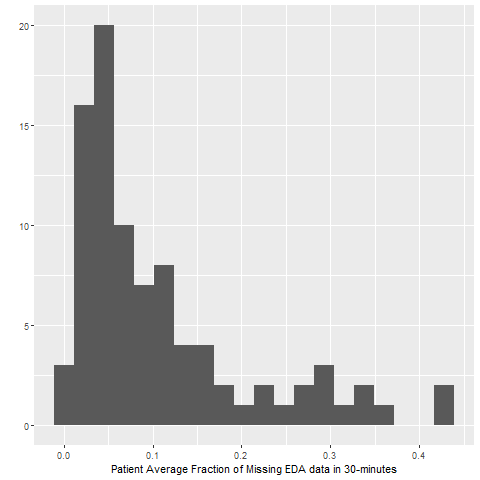
\includegraphics[width=.8\linewidth]{../figures/missing_data_eda.png}
  \caption{Electrodermal activity (EDA)}
  \label{fig:missing_eda}
\end{subfigure}%
\begin{subfigure}{.5\textwidth}
  \centering
  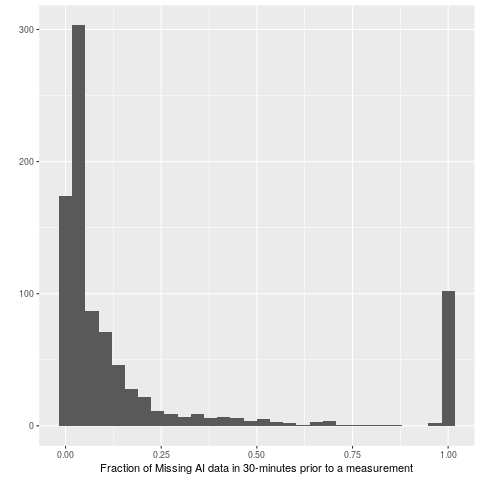
\includegraphics[width=.8\linewidth]{../figures/missing_data_ai.png}
  \caption{Activity Index (AI)
}  \label{fig:missing_acc}
\end{subfigure}
\caption{Patient average fraction missingness in 30-minute windows.}
\label{fig:mean_edacc}
\end{figure}

\newpage
\bibliographystyle{plainnat}
\bibliography{si-fda-refs}

\end{document}

